%=============================Preamble=============================%
\documentclass[10pt,a4paper]{article}
\usepackage[T1]{fontenc}
\usepackage[utf8]{inputenc}
\usepackage[brazil]{babel}
%\usepackage[math]{anttor} % fonte um pouco mais estilizada
\everymath{\displaystyle}
\usepackage{import}
%\usepackage{parskip}
%=========================Packages==================================%
\usepackage{textcomp}
\usepackage{color,lscape, amsmath, hyperref, booktabs, latexsym, multicol, gensymb, lmodern, natbib, tikz, tkz-euclide, amssymb, enumitem, fancyhdr, lipsum, siunitx, setspace}
\usepackage{graphicx}

\newenvironment{Figure}
  {\par\medskip\noindent\minipage{\linewidth}}
  {\endminipage\par\medskip}

% configurações das questões, bem como: pontuação e estrutura.

\usepackage{tasks} % cria lista curta
\usepackage{exsheets} % cria questoes
\SetupExSheets[points]{name=ponto/s,number-format=\color{blue}} % define as configurações de pontuação das questões, e a cor da pontuação.

\DeclareInstance{exsheets-heading}{fancy-wp}{default}{
toc-reversed = true ,
indent-first = true ,
vscale = 2 ,
pre-code = \rule{\linewidth}{1pt} ,
post-code = \rule{\linewidth}{1pt} ,
title-format = \large\scshape\color{rgb:red,0.65;green,0.04;blue,0.07} ,
number-format = \large\bfseries\color{rgb:red,0.02;green,0.04;blue,0.48} ,
points-format = \itshape ,
points-pre-code = ( ,
points-post-code = ) ,
join =
{
number[r,B]title[l,B](.333em,0pt) ;
number[r,B]points[l,B](.333em,0pt)
} ,
attach = { main[hc,vc]number[hc,vc](0pt,0pt) }
}

%\SetupExSheets{headings=fancy-wp} % estilo diferente para o topo do enunciado com o nome " Exercício
%===========================Margins==============================%
\usepackage[top=8mm, bottom=20mm, left=8mm, right=8mm]{geometry}

%======================Cabeçalho e Rodapé========================%
\pagestyle{fancy}
\lfoot{\notaesquerda}
\cfoot{\thepage}
\rfoot{\notadireita}
%\lhead{HELLO}
%\chead{HELLO}
%\rhead{\textbf{The performance of new graduates}}
%\renewcommand{\headrulewidth}{0.4pt} %linha horizontal no topo da pagina
\renewcommand{\footrulewidth}{0.4pt} %linha horizontal no pé da pagina

\setlength\parindent{0pt}
\setlength\parskip{1.5ex}
\setlength\parsep{1.5\parskip}
%\thispagestyle{empty}%\bigskip %Rodapé na primeira pagina

\graphicspath{{figures/}} %informa a pasta em que as imagens estão
\usepackage{capt-of}%%To get the caption
\usepackage{amsmath}%
%=======================informações da atividade===============================%
\newcommand{\atv}{Lista de Exercícios 01 -- Análise Combinatória}
\newcommand{\preceptor}{Professor: Fernando Jorge}
\newcommand{\turma}{2º serie}
\newcommand{\bolsistas}{\atv \\ \preceptor}

%=====================informações de rodapé=================%
\newcommand{\notaesquerda}{Noções de Conjuntos
}
\newcommand{\notadireita}{Escola Estadual Professor Lima Castro}


\begin{document}

{\sf
  \begin{center}
     \textbf{\bolsistas
     }
  \end{center}
}\bigskip


\vspace{2mm}
\setlength{\marginparwidth}{5cm}
\small \noindent \textbf{Nome:}\hspace{0.3cm}\hrulefill \hrulefill
\hrulefill \hspace{0.1cm} 
\textbf{Número:}\hspace{0.1cm}\rule{1cm}{.1mm}


%\begin{center}
%\textsc{\Large Exercícios}    %Titulo do topo, antes de iniciar as questões
%\end{center}

	\begin{multicols}{2}

	  \setlength\columnseprule{0.6pt} % linha vertical entre as colunas
	  %\newpage %% ou \clearpage ou %% \pagebreak %% força uma quebra de pagina. caso os exercicios ocupem apenas metade de uma pagina.

    \begin{question}[type=exam]
        Existem 2 vias de locomoção de uma cidade \textit{A} para uma cidade
        \textit{B} e 3 vias de locomoção de uma cidade \textit{B} a uma
        cidade \textit{C}. De quantas maneiras pode-se ir de \textit{A} a
        \textit{C}, passando por \textit{B}?
    \end{question}

    \begin{question}[type=exam]
        De quantas maneiras diferentes pode-se vestir uma pessoa que tenha
        5 camisas, 3 calças, 2 pares de meia e 2 pares de sapato?
    \end{question}

    \begin{question}[type=exam]
        Ao lançarmos sucessivamente 3 moedas diferentes, quantas e quais
        são as possibilidades de resultado?
    \end{question}

    \begin{question}[type=exam]
        Em um restaurante há 5 tipos de salada, 4 tipos de pratos quentes e
        3 tipos de sobremesa. De quantas maneiras podemos fazer uma refeição
        composta de 1 salada, 1 prato quente e 1 sobremesa?
    \end{question}

    \begin{question}[type=exam]
        Quantos números de dois algarismos podemos formar sabendo que o
        algarismo das dezenas corresponde a um múltiplo de 2 (diferente de zero)
        e o algarismo das unidades corresponde a um múltiplo de 3?
    \end{question}

    \begin{question}[type=exam]
        Usando somente os algarismos 1,2,3,4,5 e 6, quantos números:
        \begin{tasks}
            \task de 2 algarismos podemos formar?
            \task pares de 2 algarismos podemos formar?
            \task ímpares de 2 algarismos podemos formar?
            \task de 2 algarismos distintos podemos formar?
            \task de 2 algarismos pares podemos formar?
        \end{tasks}
    \end{question}

    \begin{question}[type=exam]
        Uma prova é composta de 7 questões do tipo "Verdadeiro ou Falso". De
        quantas maneiras um aluno pode responder a essa prova aleatoriamente,
        ou seja, "churtando" as respostas?
    \end{question}

    \begin{question}[type=exam]
        Em um salão de festas há 6 janelas. De quantas maneiras podemos escolher
        quais janelas estarão abertas ou fechadas, de modo que pelo menos uma das
        janelas esteja aberta?
    \end{question}

    \begin{question}[type=exam]
        Em uma prova de vestibular com 90 questões do tipo teste, cada questão
        tem 5 alternativas. O aluno deve preencher um cartão de respostas,
        assinalando o quadradinho correspondente à resposta de cada questão.
      \begin{Figure}
        \centering
        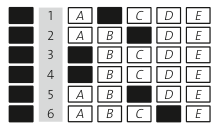
\includegraphics[scale=.7]{figures/q9.png}
      \end{Figure}
      De quantas maneiras diferentes o cartão de respostas com as 90 questões
      dessa prova poderá ser preenchido aleatoriamente? (Suponha que todas as
      90 questões foram respondidas no cartão).
    \end{question}

    \begin{question}[type=exam]
        Calcule o valor ou simplifique:
        \begin{tasks}(2)
            \task $6!$
            \task $\frac{7!}{4!}$
            \task $\frac{3!5!}{4!6!}$
            \task $\frac{n!}{(n - 2)!}$
            \task $\frac{(n+1)!}{(n+2)!}$
            \task $\frac{(n+3)!}{(n-2)!} \cdot \frac{(n-1)!}{(n+2)!}$
        \end{tasks}
    \end{question}

    \begin{question}[type=exam]
        Determine o valor de \textit{n} nas equações:
        \begin{tasks}
            \task $\frac{n!}{(n-2)} = 56$
            \task $(n+2)! + (n+1)! = 15n!$
        \end{tasks}

    \begin{question}[type=exam]
        Quantas palavras (com significado ou não) de 3 letras podemos formar
        com as letras \textbf{A}, \textbf{L} e \textbf{I}? Quais são as
        palavras?
    \end{question}

    \begin{question}[type=exam]
        Quantos números de 4 algarismos podemos escrever com os algarismos
        2,4,6,8? E de 4 algarismos distintos?
    \end{question}

    \begin{question}[type=exam]
        De quantas maneiras uma família de 5 pessoas pode se sentar em um
        banco de 5 lugares para tirar uma foto?
      \end{question}

    \begin{question}[type=exam]
        Quantos são os anagramas da palavra \textbf{AMOR}?
    \end{question}

    \begin{question}[type=exam]
        Quantos números naturais de algarismos distintos entre 5000 e 10000
        podemos formar com os algarismos 1,2,4 e 6?
      \end{question}

    \begin{question}[type=exam]
        Considere todos os anagramas da palavra TEORIA.
        \begin{tasks}
            \task Quantos são?
            \task Quantos começam por TEO?
            \task Quantos têm as letras TEO juntas nessa ordem?
            \task Quantas têm as letras TEO juntas em qualquer ordem?
            \task Quantos têm as vogais juntas, em ordem alfabética, e as
            consoantes juntas, em qualquer ordem?
        \end{tasks}
    \end{question}

    \begin{question}[type=exam]
        Colocando todos os anagramas da palavra \textbf{AMIGO} listados em
        ordem alfabética, como em um dicionário, qual será a:
        \begin{tasks}
        \task $1^\circ$ palavra?
        \task $2^\circ$ palavra?
        \task $25^\circ$ palavra?
        \task penúltima palavra?
        \task $55^\circ$ palavra?
        \end{tasks}
    \end{question}

		\clearpage
	\end{multicols}

  %\import{questions/}{q7} % exemplo para mostrar que pode colocar questões fora das colunas e mesclar os estilos. Recomendado adicionar questões que incluem imagens, ao final e fora das colunas.






\end{document}
